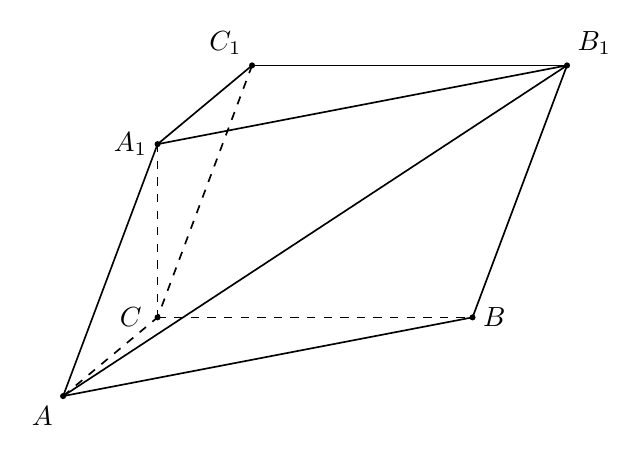
\begin{tikzpicture}[line width=0.6pt, font=\normalsize]
  \coordinate (A) at (0,0);
  \coordinate (C) at (1.2,1.0);
  \coordinate (B) at (5.2,1.0);
  \coordinate (A1) at (1.2,3.2);
  \coordinate (C1) at (2.4,4.2);
  \coordinate (B1) at (6.4,4.2);
  % base
  \draw (A) -- (B);
  \draw[dashed] (C) -- (B);
  % laterals and top
  \draw (A) -- (A1);
  \draw (A) -- (B1);
  \draw (A1) -- (B1);
  \draw (B) -- (B1);
  \draw (C1) -- (B1);
  \draw (A1) -- (C1);
  \draw[dashed] (A1) -- (C);
  \draw[dashed] (C1) -- (C);
  \draw[dashed] (A) -- (C);
  \foreach \p in {A,B,C,A1,C1,B1} {\fill (\p) circle (1.1pt);}
  \node[below left=2pt, inner sep=1.5pt] at (A) {$A$};
  \node[right=2pt, inner sep=1.5pt] at (B) {$B$};
  \node[left=2pt, inner sep=1.5pt,xshift=-2.00bp,yshift=0.00bp] at (C) {$C$};
  \node[left=2pt, inner sep=1.5pt] at (A1) {$A_{1}$};
  \node[above left=2pt, inner sep=1.5pt] at (C1) {$C_{1}$};
  \node[above right=2pt, inner sep=1.5pt] at (B1) {$B_{1}$};
\end{tikzpicture}
